\chapter{Implementations}
\label{Implementations}

\epigraph{\textit{Unperformed experiments have no results}}{Asher Peres}

%%% intro
\section{Not another introduction!}
\begin{comment}
Classical computers are ubiquitous in today's society. They are present in nearly every electronic device, from embedded microcontrollers in washing machines and fridges, through microprocessors in mobile phones and computers, all the way to large scale servers and mainframes controlling critical infrastructure and powering the internet. 

Three features of computers make this possible: the ability to pack millions of transistors into a single silicon die; the extremely small cost of doing it; and the existence of software that abstract away implementation details.
\end{comment}

The vast majority of tasks facing modern programmers require little or no knowledge of how computers really work. There is a wealth of of programming languages and development tools which remove implementation details and allow the engineer to focus on the important aspects of the task at hand.

However, in the general quest to develop a quantum computer, it pays to take a closer look at the internal structure of computers. The language surrounding quantum algorithms has been heavily influenced by classical computers (the most important example being the qubit, which is analogous to a classical bit), and it makes sense that the implementation of a large scale quantum computer might be similarly influenced by its classical counterpart. Furthermore, due to the lack of large scale quantum computers, complex software stacks and quantum development environment which hide implementation details simply do not exist.

We therefore consider it necessary to understand at least the basics of how quantum computers might work. In this section, we discuss possible architectures of future large scale quantum computers. In particular, we consider the similarities and differences between classical and quantum computers, and how this might lead to differences between classical and quantum programming languages.

The section is divided into two main parts. The first focuses on quantum computer hardware and the physical systems which represent qubits and implement quantum operations. The second is focused on the implementation of quantum algorithms, from the instruction set level up to high level languages.

\begin{comment}
We begin with a brief review of the historical development of computers and software, which we use as the starting point for our discussion of quantum computer architectures. Then we discuss quantum computer hardware, and briefly outline a few of the current approaches to quantum computer design. Finally, we consider how quantum languages might be designed if a large scale quantum computer did in fact exist.
\end{comment}

% classical computers
\subsection{The development of classical computers}

\begin{comment}
Are classical computers optimal? If it we had access to all the technology and hindsight we have now, would computers have developed differently? How would you optimally arrange a billion transistors into a classical computer if you could start from scratch?

There are many different approaches to computation. Some devices, such as the abacus or slide rule, are simple mechanical devices that speed up certain operations (performing arithmetic and finding logarithms)  Others, such as Charles Babbage's difference engine, which computes polynomial approximates to logarithmic and trigonometric functions it also operates using mechanical means. However, the mechanism is automated so

Following the invention of the transistor in the late 1940s, 

These are the problems we face in the design of a quantum computer today. We have an opportunity to consider these questions now, in anticipation of the existence of a billion qubit quantum computer.

The fundamental unit in the modern classical computer is the transistor. However, the transistor did not mark the beginning of the development of computers.
-------------- PLAN ---------------

Babbage difference engine -- calculation of polynomial expressions, based on full adder operations realised 
analog computing -- solving differential equations with op amps.
The general purpose computer -- turing machines, etc
Von Neumann paper on computer architecture
Digital computers using transistors

quantum computers as something different to a computer -- perhaps it's wrong to draw any analogy at all.

Is it possible to learn from the development of computers? Make standards to avoid the back compatibility problems in classical; think about a universal optimal architecture, etc.

How did computers develop? Development of transistors, logic, the microcontroller, the minicomputer, etc. Comparison of different types of architectures: Harvard, Von-Neuman, transputers(!) (to make the point that some of them failed!). Suggestions of where we are at with quantum computer development -- maybe transistors/logic gates.
\end{comment}

% Quantum computer architecture
\section{Quantum computer hardware architecture}

Quantum architecture is to do with the structures that make up a quantum computer: there need to be qubits, unitary operations (data processing), memory (data storage), control (instruction execution), `buses' (getting enough connectivity between qubits), input/output (quantum measurement, initialising qubits), error correction (preventing decoherence of quantum states). Several architecture features are achieved by using ancilla qubits (qubits required to implement certain useful operations). 

In this section we would like to compare the architecture of a quantum computer with the architecture of a classical computer. Most high level elements are analogous, but there are some differences: e.g. error correction is not thought of in the same way classically. Most of the elements are subtly different: quantum I/O involves quantum measurements; memory basically involves swapping qubits since copying is not allowed.

Quantum instruction sets (a higher level type of architecture) can be made analogous to classical instruction sets in terms of their purpose (to expose fundamental units of data processing and control to a compiler).

\begin{figure}[H]
    \centering
    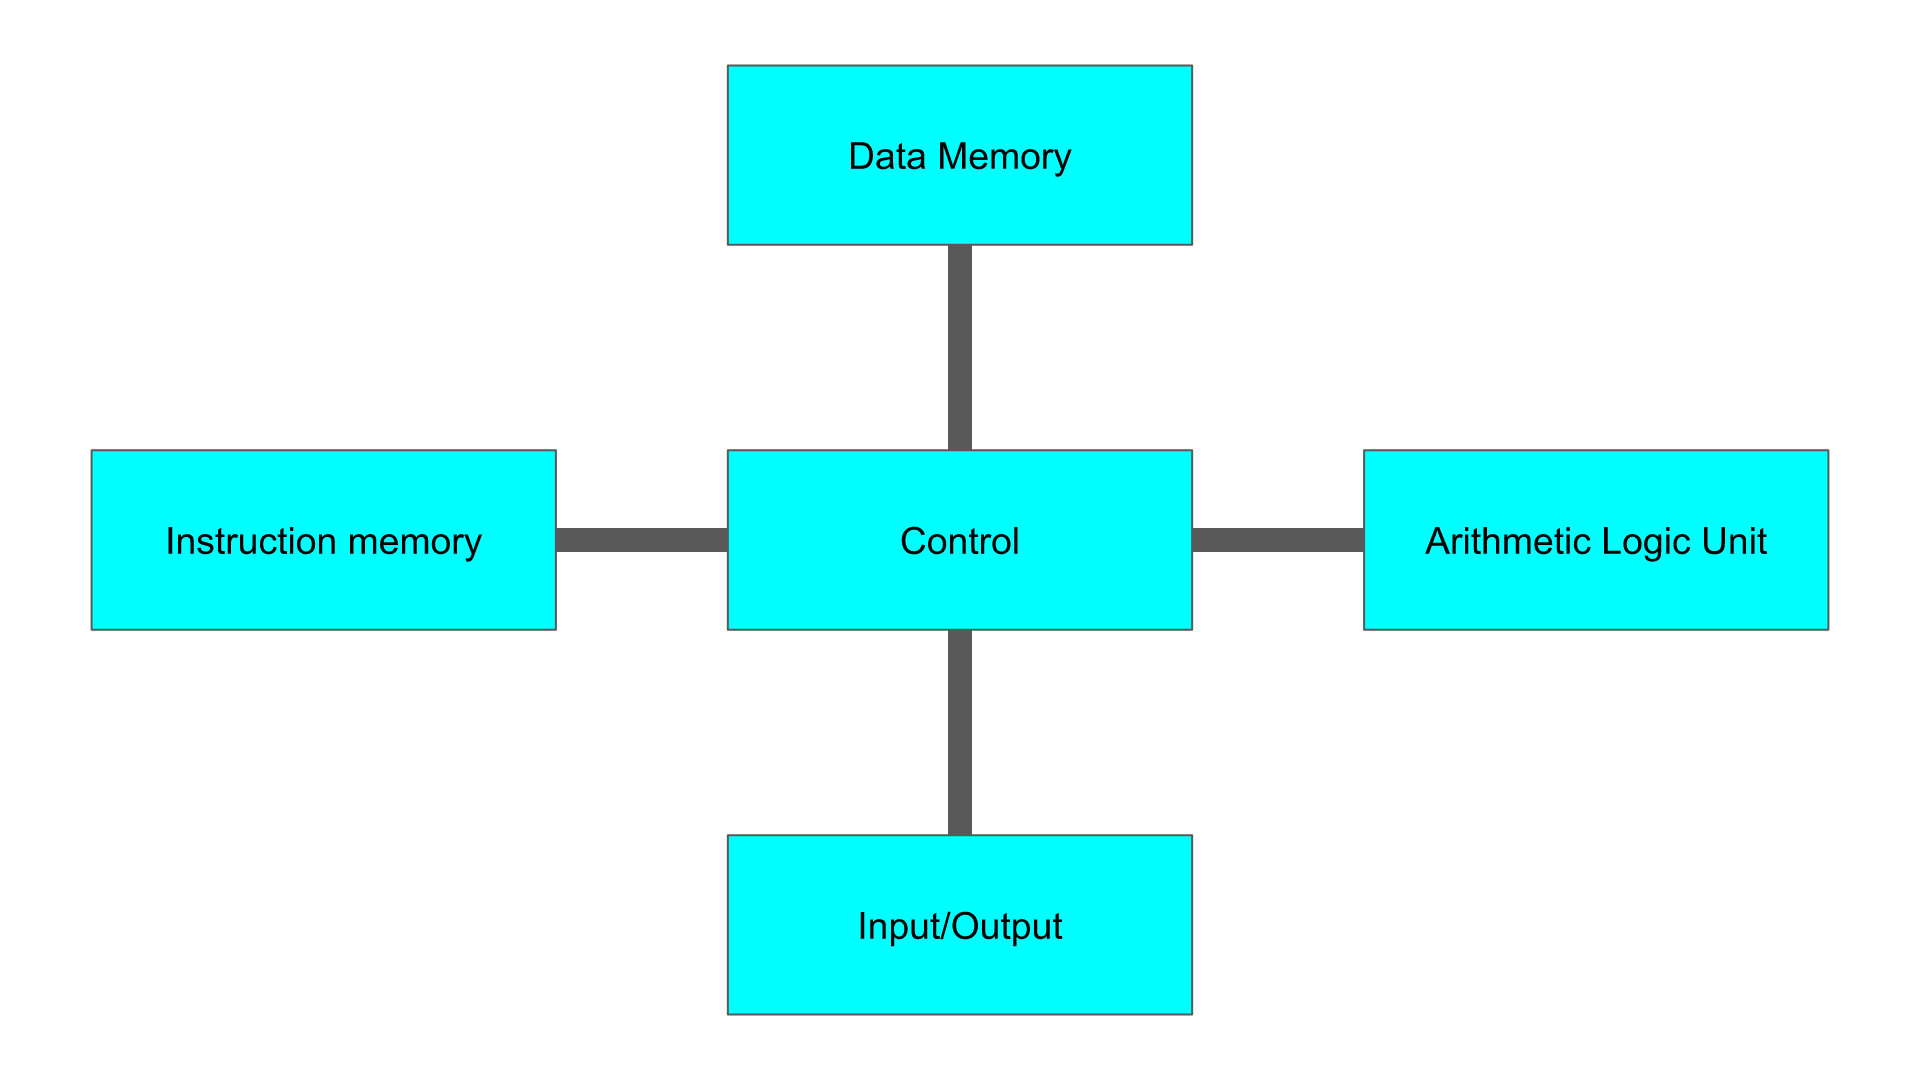
\includegraphics[width=0.8\textwidth]{figures/impl/harvardarch.png}
    \caption{Harvard Architecture}
    \label{fig:cpuHarvArch}
\end{figure}

The over-arching structure for quantum computers can be separated into two parts, there is the architecture and the platform. A quantum architecture has a different meaning to the traditional use of the word. Within the community, architectures is the distinction between the gate model, one-way quantum computing or topological quantum computing. A platform is the physical system that is used to build the computer such as, photonics, trapped ions, semi-conductor qubits, super-conducting qubits. 

We now discuss some of the current physical approaches to building a quantum computer. In reality the quantum architectures and platforms are not completely separate, some physical systems are much better suited to specific architectures. For example the gate model is a natural choice when using trapped ions or superconducting qubits whereas photons are much better suited to one-way quantum computing. 

There are two distinct types of qubits, stationary (e.g. Trapped ions or superconducting qubits) or flying qubits (photons). Here we will only discuss trapped ions and photons \textbf{Poisson Bullets are the best!!1!} as we believe these systems are the easiest to visualise conceptually. 

A good way to think of a quantum computer is a very large, noisy machine which is incredibly sensitive to its environment. The aim is trying to control it just to keep the machine coherent. Most of the resources used are for error correction, keeping the whole thing coherent, a very small part of the whole machine is the information processing. 

% what are the qubits
\subsection{What are the qubits?}

\subsection{What are the operations?}

%%%%%%%%%%%%%%%%%%%%%%%%%%%%%%%%%%%%%%%%5555
\subsection{Trapped Ions}

Trapped ions are a remarkably stable physical system (once an ion is trapped it remains trapped with a very high probability). Electric fields are used to trap the ions, by changing the voltages in the x,y,z components in the electric field it is possible to shuttle the individual ions around. This enables a great deal of control over the dynamics of the ions.

The quantum gates are performed on the qubits using either microwaves which use atomic transitions or optical pulses for electronic transitions. The microwave gates are appealing as it opens the possibility of addressing multiple qubits at once. This will be necessary when taking into account error correction as one logical X operation could correspond to 100s or 1000s of X operations on physical qubits to produce one logical X. 

The \cite{lekitsch2015blueprint} blueprint suggests using a modular approach of packing tiles shown in \autoref{fig:iontrap} on a 2D surface. Each tile would contain one ion and have a dedicated loading zone, an entangling zone with adjacent tiles each with only one ion on and a detection zone for readout. Entangling gates or operations are performed by bringing two qubits close together. This is relatively easy for trapped ions as of the good control available. 

\begin{figure}[h]
    \centering
    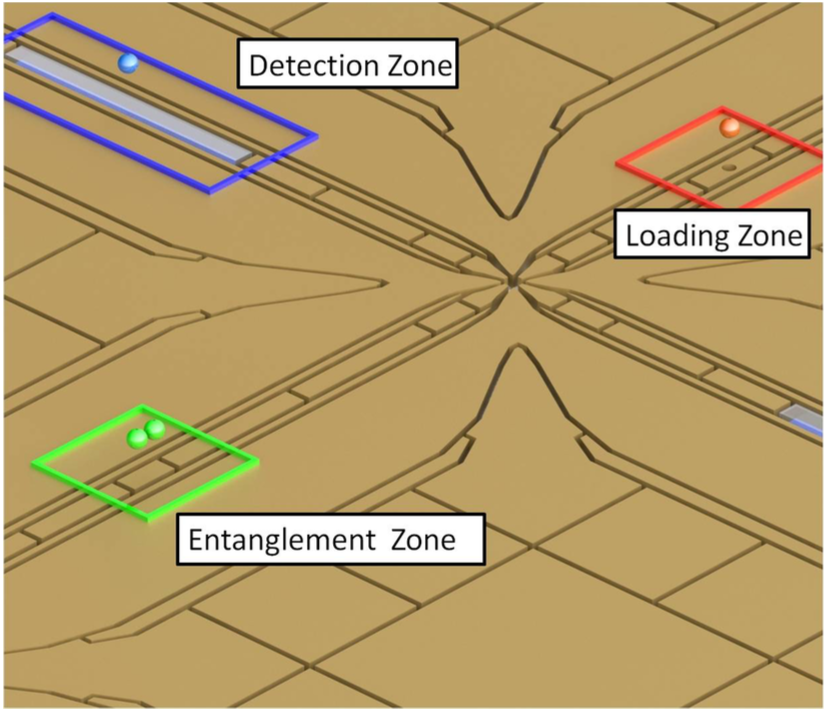
\includegraphics[width=0.6\textwidth]{figures/impl/iontrap.png}
    \caption{Caption \cite{lekitsch2015blueprint}}
    \label{fig:iontrap}
\end{figure}

%%%%%%%%%%%%%%%%%%%%%%%%%%%%%%%%%%%%%%%%%%%
\subsection{Superconducting qubits}


%%%%%%%%%%%%%%%%%%%%%%%%%%%%%%%%%%%%%%%%%%%%
\subsection{Linear optical quantum computing}

linear optical quantum computing is great! 

\begin{figure}[h]
    \centering
    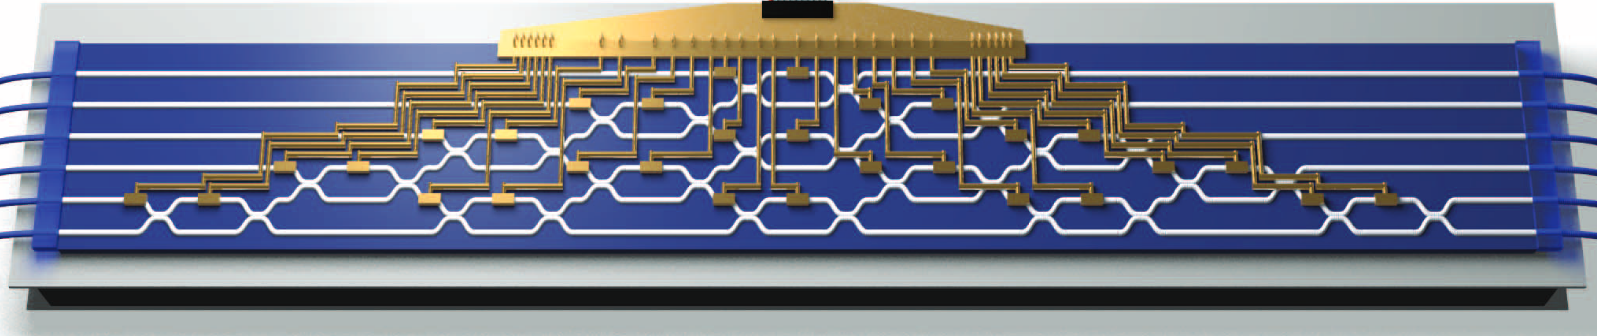
\includegraphics[width=0.6\textwidth]{figures/impl/rekkchip.png}
    \caption{Caption \cite{carolan2015universal}}
    \label{fig:my_label}
\end{figure}


%%%%%%%%%%%%%%%%%%%%%%%%%%%%%%%%%%%%%%%%%%%%
\subsection{Error Correction}

Full fault tolerance is beyond the scope of this guide however we will briefly discuss error correction. The basic idea of error correction is to use redundancy to counteract errors. Increasing the resources devoted to storing the logical information should in principle make the computer more resilient to errors.


\begin{comment}
--- PLAN ---

Focus on implementation of quantum programming languages

Implementing quantum computers:
\begin{itemize}
\item Comparison of quantum and classical computer architectures
Classical computer architectures: ALU, CPU, buses, memory, instructions, etc equivalents for quantum computers? Quantum architectures: gates? Cluster states? Quantum vs. Classical control? What are the analogues of instructions, execution, buses and memory? Are there fundamental limits to architecture design (imposed by eg no cloning. Does memory make sense in the same way as for classical computers? Quantum memory is more like single-use working-registers). How about classical computers with quantum instructions? What about qbranch instructions?   
\item Different quantum computing platforms 
Probably just a few -- maybe linear optical quantum computers and iron traps. 
\item Classical language compilers
\end{itemize}
Implementing quantum programming:
\begin{itemize}
\item Quantum error correction
Not entirely analogous to classical computers, (no instruction execution errors). Can error correction be abstracted away from the compiler level? Would error correction take place at the equivalent level of (say) instruction pipe lining in a classical processor?    
\item Quantum language compilers
What is the quantum equivalent of object code? Does it contain machine code (instructions to be executed, analogous to classical computers) or does it compile into an arrangement of gates, or some other computation mode (measurements in a cluster state?). The architecture of the quantum computer would probably heavily inform the structure of low level languages. (For example, C has basic structures essentially based on mov, branch, and arithmetic and bit manipulation instructions). Hence the low level languages of gate based quantum computers will be based on structures easily realised using gates (the gates themselves, presumably analogous to bit manipulation; coherent arithmetic, (implemented using gate arrangements lifted from half and full adders); flow control -- presumably classical; and strict mov operations, ie excluding copy). Low level languages targeted at cluster state implementation will have cluster state measurements as primitive operations (equivalent to bit manipulation) in the language, and presumably various other generic operations (like control, branching, etc.) What kind of optimisations does the C compiler do, and what are the equivalents in the quantum cases? 
\end{itemize}
--- PLAN ---
\end{comment}